\documentclass{article}
\usepackage[utf8]{inputenc}
\usepackage{physics}
\usepackage{xcolor}
\usepackage{graphicx}
\definecolor{codegray}{rgb}{0.9,0.9,0.9}
\usepackage{listings}
\newcommand{\morpho}{\textit{morpho}}
\newcommand{\Morpho}{\textit{Morpho}}
\title{Q-tensor model of nematics}
\author{Chaitanya Joshi}
\date{October 2021}

\begin{document}
\lstset{  
language=Java,  
tabsize=4,  
basicstyle=\ttfamily,  
backgroundcolor=\color{codegray},  
showstringspaces=false  
}
\maketitle

\section{Introduction}
In 2D, for a uniaxial nematic, we can define a Q-tensor:
\[
Q_{ij} = S (n_i n_j - 1/2 \delta_{ij})
\]
Here, the $-1/2 \delta_{ij}$ is added for convenience, to make the matrix traceless: 
\[\text{Tr}(\mathbf{Q}) = Q_{ii} = S(n_i n_i - 1/2 \delta_{ii}) = S(1 - 1/2(2)) = 0
\]
Now, the Q-tensor is also symmetric by definition:
\[
Q_{ij} = Q_{ji}
\]
Due to these two reasons we can write the Q-tensor as a function of only $Q_{xx}$ and $Q_{xy}$:
\[
\mathbf{Q} = \begin{bmatrix}Q_{xx} & Q_{xy} \\ Q_{xy} & -Q_{xx} \end{bmatrix}
\]
\subsection{Simple Passive Nematic Model}
The Landau-de Gennes equilibrium free energy for a nematic liquid crystal can be written in terms of the Q-tensor:
\begin{align*}
F_{LDG} = &\int_\Omega d^2{\bf x} \ \left(\frac{a_2}{2} \text{Tr}(\mathbf{Q}^2) + \frac{a_4}{4} (\text{Tr} \mathbf{Q}^2)^2 + \frac{K}{2}(\nabla\mathbf{Q})^2 \right) \\
&+ \oint_{\partial\Omega} d{\bf x} \frac{1}{2}E_A \text{Tr}[(\mathbf{Q}-\mathbf{W})^2]
\end{align*}
where $a_2 = (\rho-1)$ and $a_4 = (\rho+1)/\rho^2$ 
set the isotropic to nematic transition with $\rho$ being the non-dimensional density. The system is in the isotropic state for $\rho<1$ and in the nematic phase when $\rho>1$. In the nematic phase, $\ell_n = \sqrt{K/a_2}$ sets the nematic coherence length. Now,
\[
\mathbf{Q}^2 = \begin{bmatrix}Q_{xx} & Q_{xy} \\ Q_{xy} & -Q_{xx} \end{bmatrix} \begin{bmatrix}Q_{xx} & Q_{xy} \\ Q_{xy} & -Q_{xx} \end{bmatrix} = (Q_{xx}^2+Q_{xy}^2) \begin{bmatrix} 1 & 0 \\ 0 & 1 \end{bmatrix}
\]
Hence, 
\[
\text{Tr}(\mathbf{Q}^2) = 2(Q_{xx}^2+Q_{xy}^2)
\]
Similarly,
\[
(\nabla \mathbf{Q})^2 = \partial_i Q_{kj}\partial_i Q_{kj} = 2 \{ (\partial_x Q_{xx})^2+(\partial_xQ_{xy})^2 + (\partial_y Q_{xx})^2+(\partial_y Q_{xy})^2 \}
\]
Now, the second term is a boundary integral, with $E_A$ being the anchoring strength. $\mathbf{W}$ is the tensor corresponding to the boundary condition. For instance, for parallel anchoring, 
\[
W_{ij} = (t_i t_j - 1/2 \delta_{ij})
\]
where $t_i$ is a component of the tangent vector at the boundary.
$\mathbf{W}$ is also a symmetric traceless tensor with two independent components $W_{xx}$ and $W_{xy}$.
The boundary term becomes:
\[ \text{Tr}[(\mathbf{Q}-\mathbf{W})^2] = 2\{ Q_{xx}^2 + Q_{xy}^2 - 2(Q_{xx}W_{xx} + Q_{xy}W_{xy}) + W_{xx}^2 + W_{xy}^2 \} 
\]
\section{Vector formulation}
We can formulate all these expressions in terms of vector quantities:
\[\vec{q} \equiv \{ Q_{xx}, Q_{xy}\}\]
\[\vec{w} \equiv \{ w_{xx}, w_{xy}\}\]
Thus,
\[
\text{Tr}(\mathbf{Q}^2) = 2 ||\vec{q}||^2
\]

\[
(\nabla \mathbf{Q})^2 = 2 ||\nabla \vec{q}||^2
\]

\[
\text{Tr}[(\mathbf{Q}-\mathbf{W})^2] = 2 ||\vec{q}-\vec{w}||^2
\]
With these, we want to minimize the area-integral of 
\[
F = \int_\Omega d^2{\bf x} \ \left( a_2 ||\vec{q}||^2 + a_4 ||\vec{q}||^4 + K||\nabla\vec{q}||^2 \right)
\]
together with the line-integral energy
\[
\oint_{\partial\Omega} d{\bf x} \ E_A ||\vec{q}-\vec{w}||^2
\]

\section{\Morpho \ implementation}
This free energy is readily set up in \morpho. For this problem, we will consider a 2D disk geometry with unit radius. We use $\rho=1.3$, so that we are deep in the nematic regime. We fix $E_{\text{A}}=3$, which sets strong anchoring at the boundary. With this strong tangential anchoring, we get a topological charge of $+1$ at the boundary, and this acts as a constraint. When the nematic coherence length is comparable to the disk diameter ($\ell_n \sim R$), the $+1$ charge penetrates throughout the disk, whereas if ($\ell_n \ll R$), then a formation with 2 $+1/2$ defects is more stable. To test this, we use two different values of $K$:, 0.01 and 1.0.

We first define all our parameters and import $\texttt{disk.mesh}$ from the tactoid example:
\begin{lstlisting}
var rho = 1.3 // Deep in the nematic phase
var EA = 3 // Anchoring strength
var K = 0.01 // Bending modulus

var a2 = (1-rho)
var a4 = (1+rho)/rho^2

var m = Mesh("disk.mesh")
var m = refinemesh(m) // Refining for a better result
var bnd = Selection(m, boundary=true)
bnd.addgrade(0) // add point elements

\end{lstlisting}
We define the Q-tensor in its vector form as discussed above, initializing it to small random values:
\begin{lstlisting}
var q_tensor = Field(m, fn(x,y,z)
Matrix([0.01*random(1), 0.01*random(1)]))
\end{lstlisting}
Note that this incidentally makes the director parallel to a 45 degree line. 
We now define the bulk energy, the anchoring energy and the distortion free energy as follows:
\begin{lstlisting}
// Define bulk free energy
fn landau(x, q) {
  var qt = q.norm()
  var qt2=qt*qt
  return a2*qt2 + a4*qt2*qt2
}
// Define anchoring energy at the boundary
fn anchoring(x, q) {
  var t = tangent()
  var wxx = t[0]*t[0]-0.5
  var wxy = t[0]*t[1]
  return (q[0]-wxx)^2+(q[1]-wxy)^2
}

var bulk = AreaIntegral(landau, q_tensor)
var anchor = LineIntegral(anchoring, q_tensor)
var elastic = GradSq(q_tensor)
\end{lstlisting}
Equipped with the energies, we define the \texttt{OptimizationProblem}:
\begin{lstlisting}
var problem = OptimizationProblem(m)
problem.addenergy(bulk)
problem.addenergy(elastic, prefactor = K)
problem.addenergy(anchor, selection=bnd, prefactor=EA)
\end{lstlisting}
To minimize the energy with respect to the field, we define the \texttt{FieldOptimizer} and perform a \texttt{linesearch}:
\begin{lstlisting}
var opt = FieldOptimizer(problem, q_tensor)
opt.linesearch(500)
\end{lstlisting}
\section{Visualizing the result}
For visualizing the final configuration, we use the same piece of code we used for the tactoid example, and define some additional helper functions to extract the director and the order from the Q-tensor.
\begin{lstlisting}
fn sign(x) {
  if (x<0.0) return -1.0
  else if (x>0.0) return 1.0
  return 0.0
}
\end{lstlisting}
\begin{lstlisting}
fn qtodirector(q) {
  var S = 2*q.norm()
  var Q = q/S
  var nx = sqrt(Q[0]+0.5)
  var ny = abs(Q[1]/nx)
  nx*=sign(Q[1])
  return Matrix([nx,ny,0])
}
\end{lstlisting}
\begin{lstlisting}
fn qtoorder(q) {
  var S = 2*q.norm()
  return S
}
\end{lstlisting}
\begin{lstlisting}
// Convert the q-tensor to the director and order
var nn = Field(m, Matrix([1,0,0]))
for (i in 0...m.count()) nn[i]=qtodirector(q_tensor[i])
var S = Field(m, 0)
for (i in 0...m.count()) S[i]=qtoorder(q_tensor[i])
\end{lstlisting}
\begin{lstlisting}
// Function to visualize a director field
fn visualize(m, nn, dl) {
  var v = m.vertexmatrix()
  var nv = v.dimensions()[1]
  var g = Graphics()
  for (i in 0...nv) {
    var x = v.column(i)
    g.display(Cylinder(x-nn[i]*dl, x+nn[i]*dl,
    aspectratio=0.3))
  }
  return g
}

// Visualize the result
// var g=plotmesh(m, grade=1)
var splot = plotfield(S, style="interpolate")
var gnn=visualize(m, nn, 0.05)
var gdisp = splot+gnn
Show(gdisp)
\end{lstlisting}
We can go further and use the \texttt{povray} module to render a \texttt{.png} output:
\begin{lstlisting}
var pov = POVRaytracer(gdisp)
pov.viewangle=35
pov.render("Qtensor_K_${K}.pov")
\end{lstlisting}
\begin{figure}
    \centering
    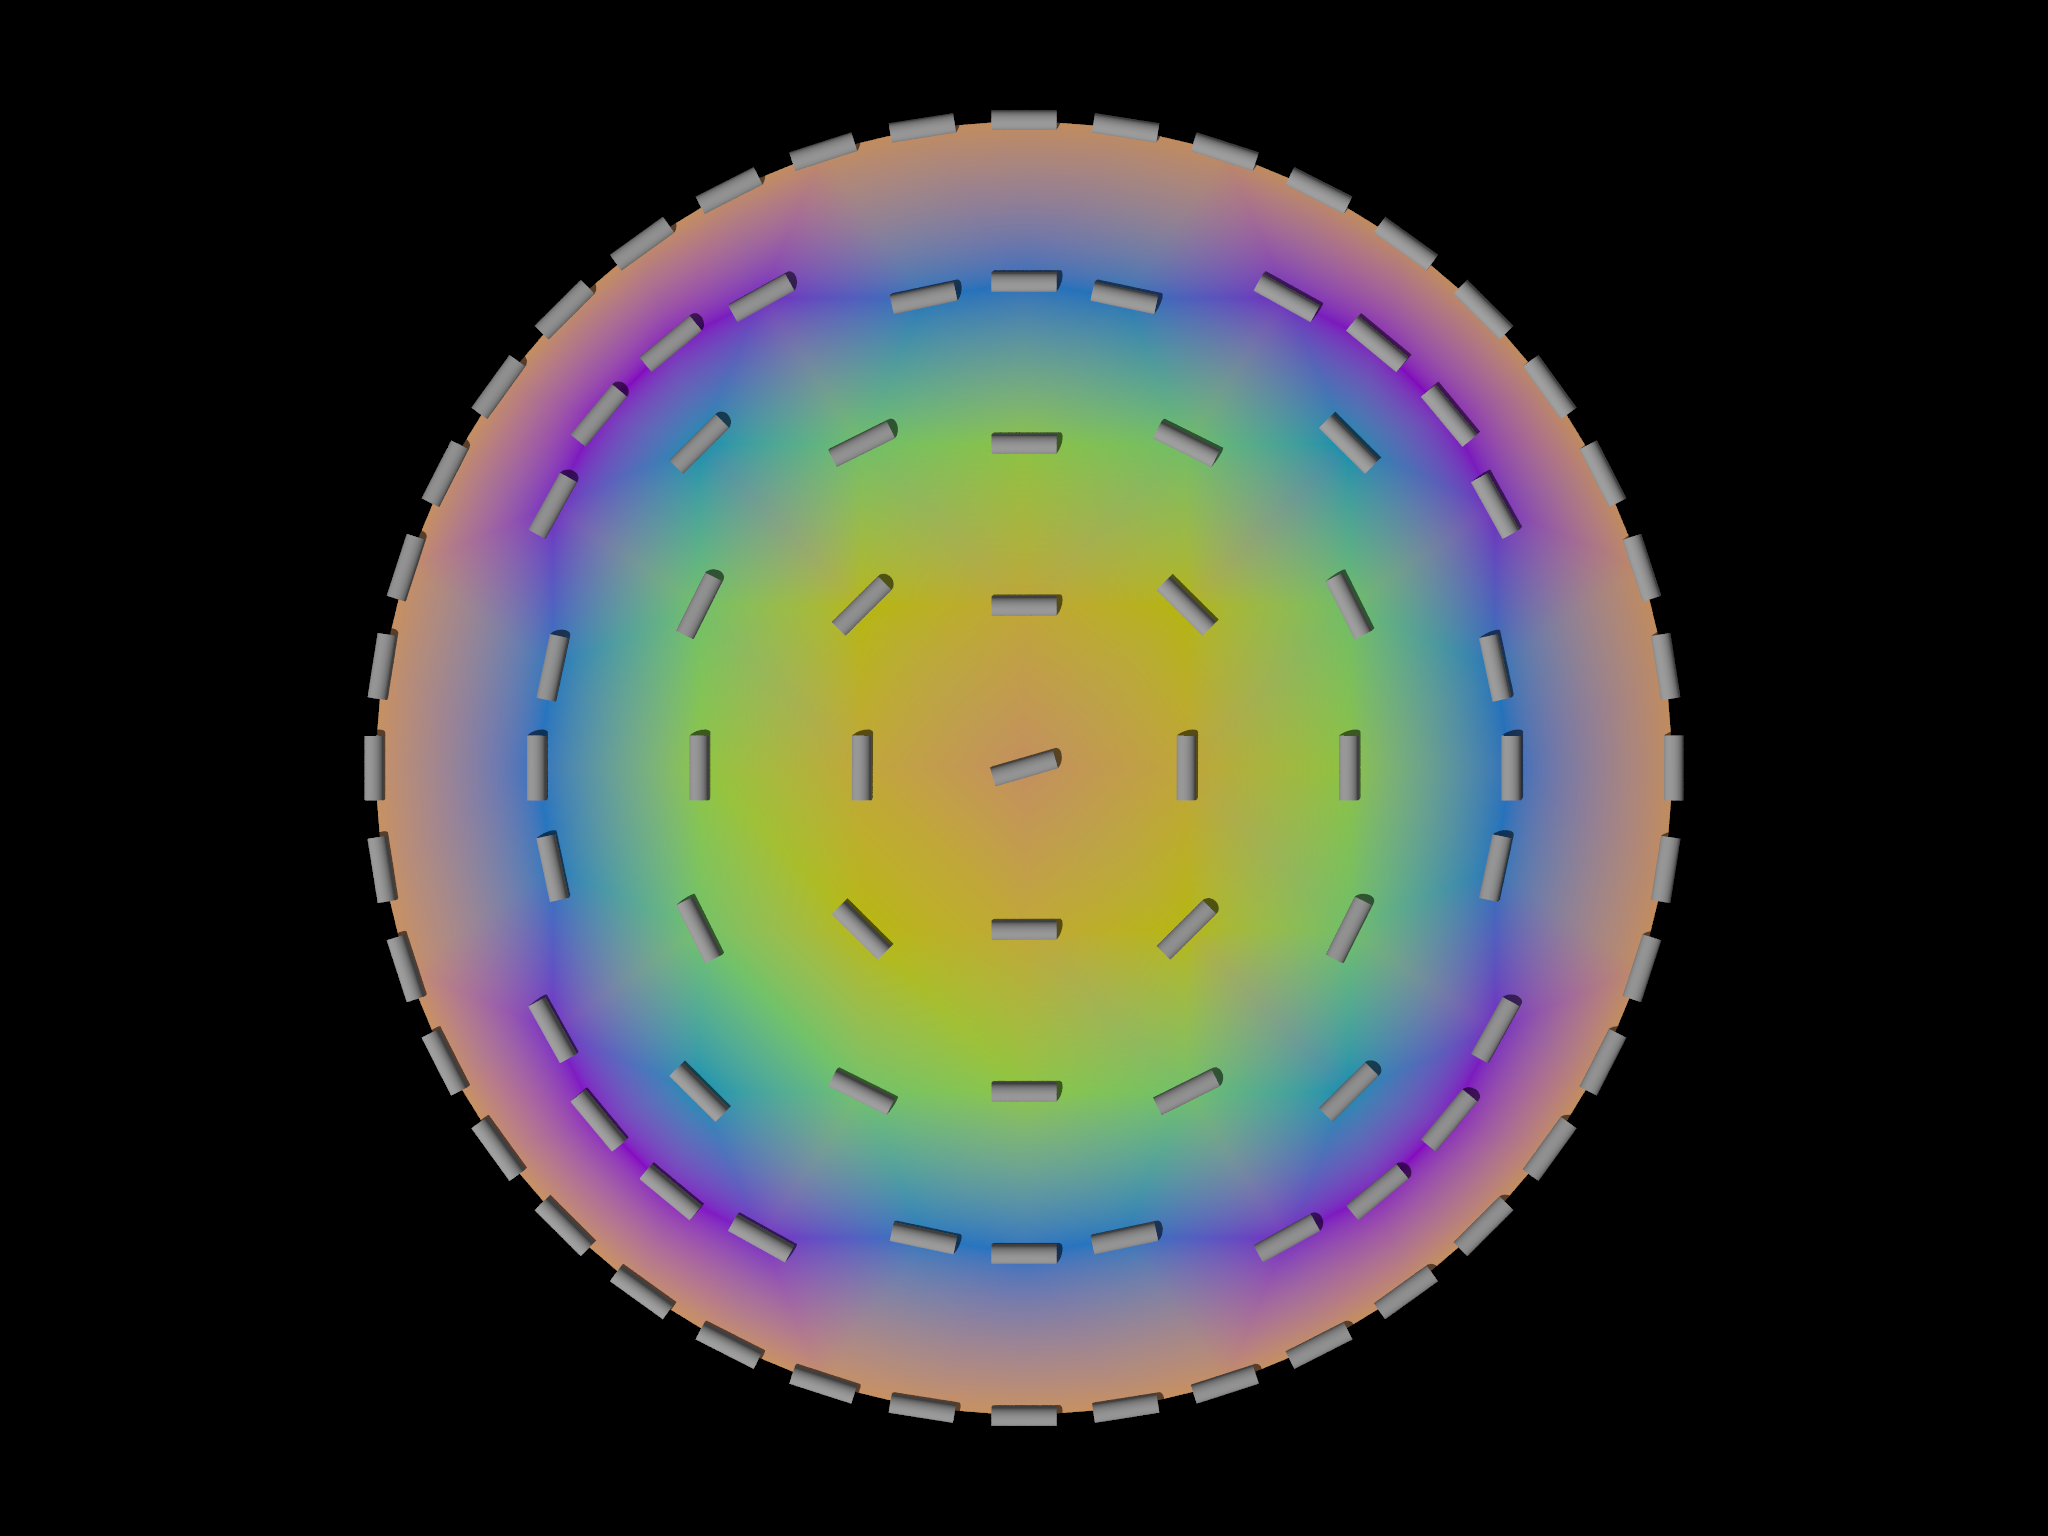
\includegraphics[width=0.45\linewidth]{Qtensor_K_1.png}
    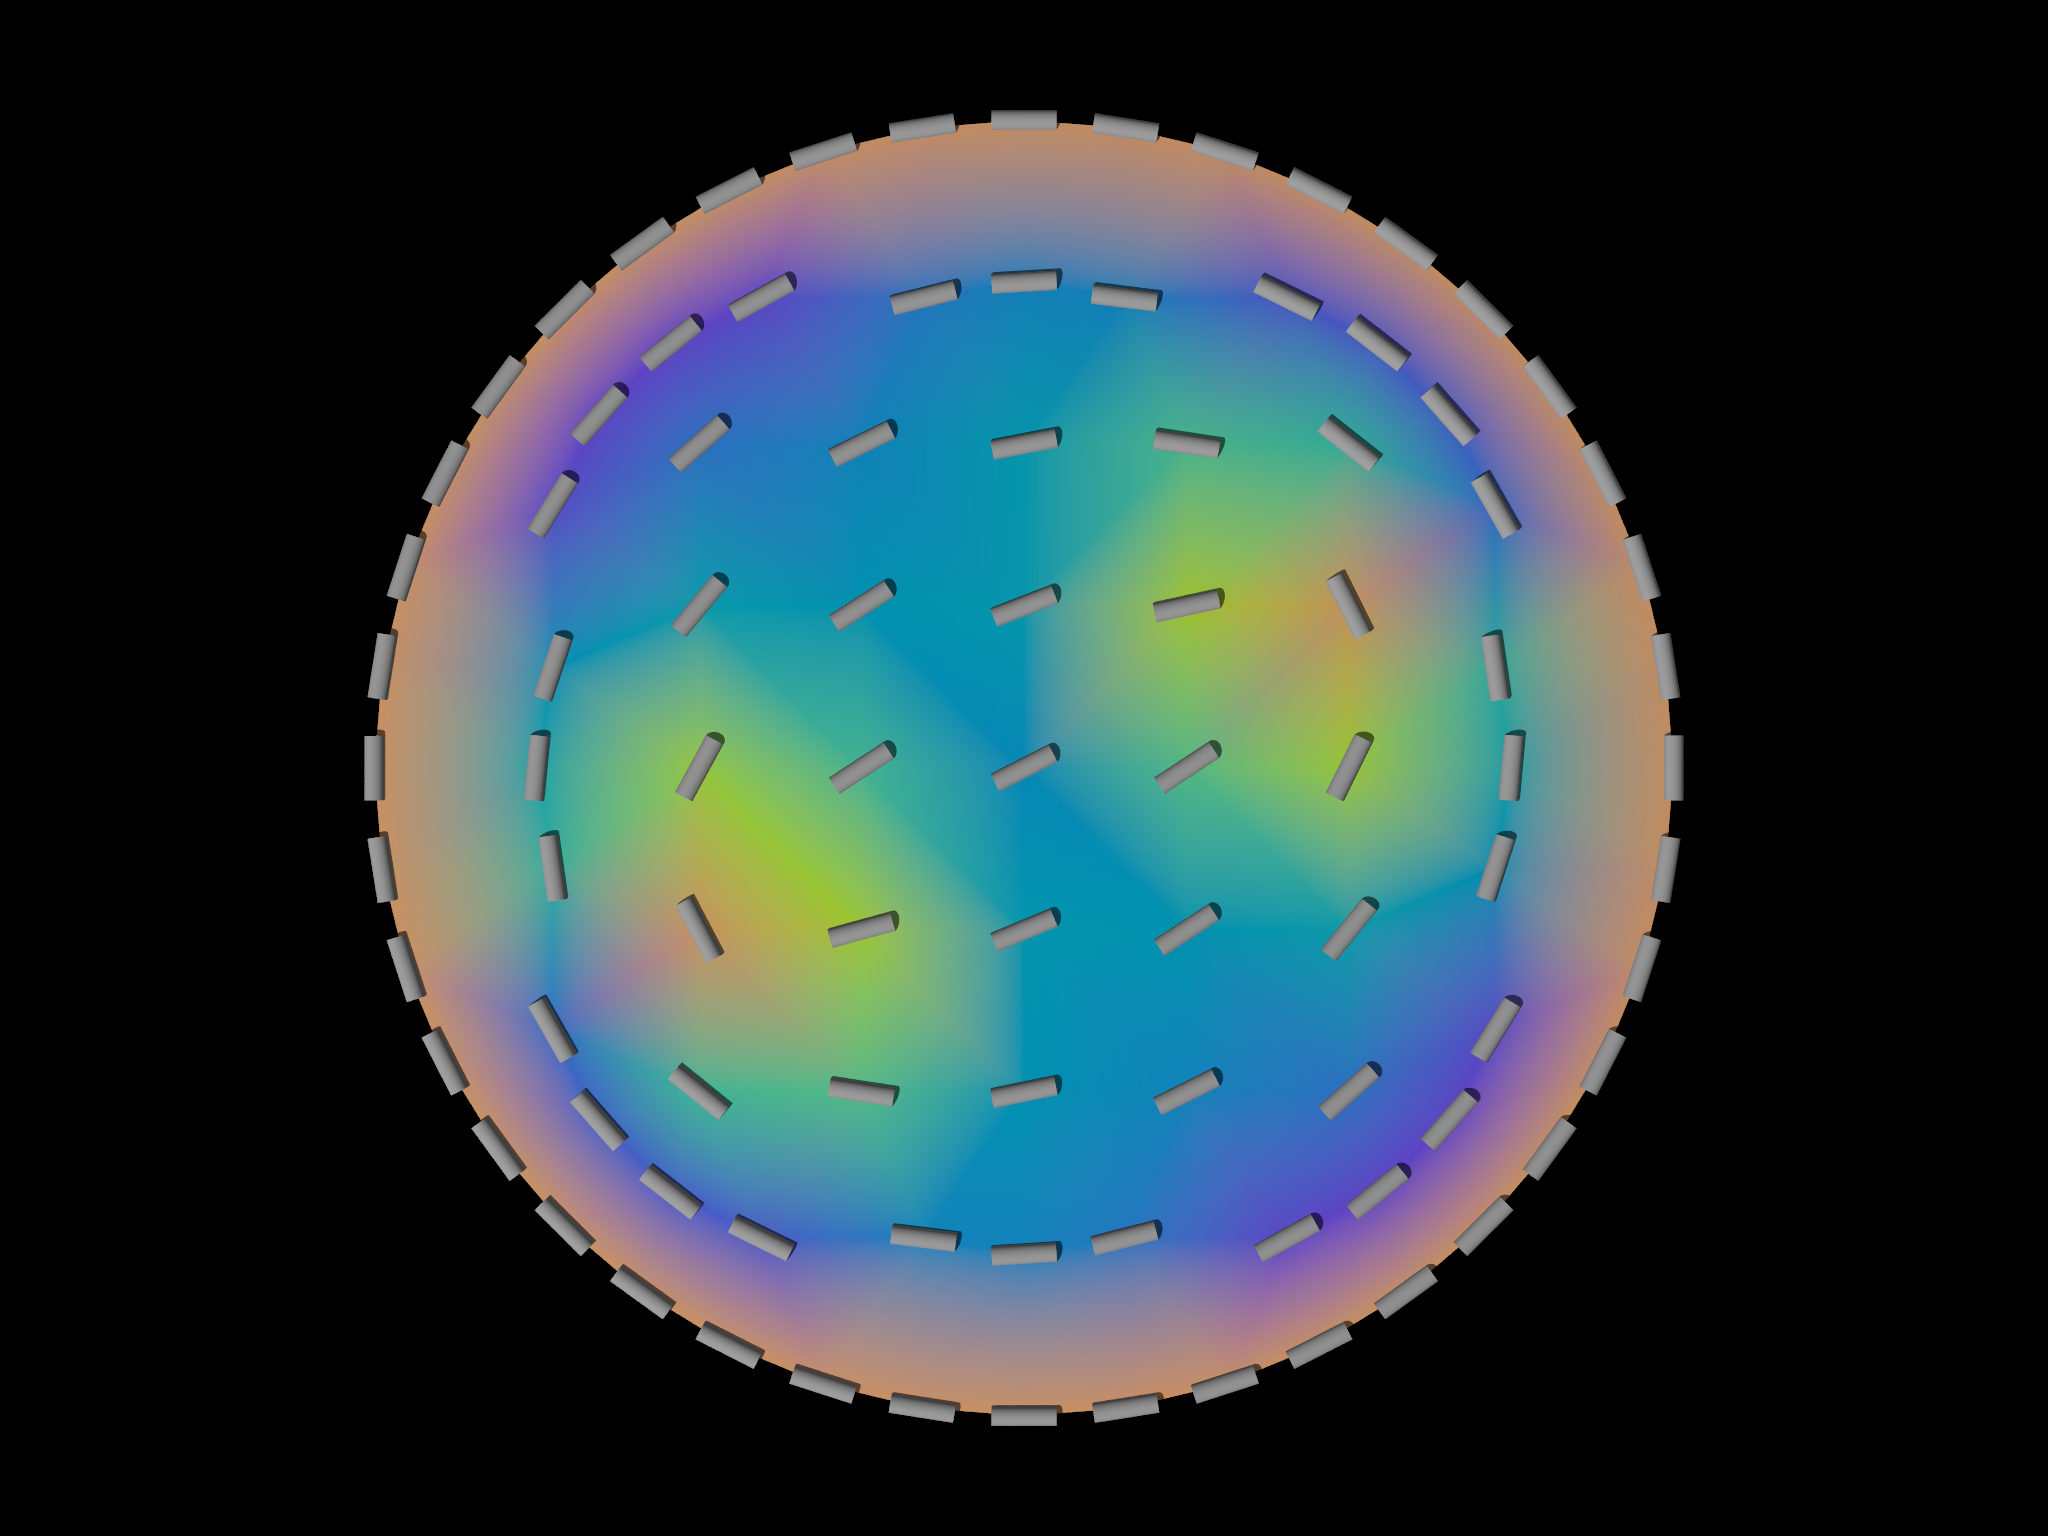
\includegraphics[width=0.45\linewidth]{Qtensor_K_0.01.png}
    \caption{Final configuration of the director and order for (left) $K=1$ and (right) $K=0.01$. The cylinders indicate the nematic director whereas the color indicates the scalar order parameter. Note how the $K=1$ case has a single $+1$ defect at the center whereas the $K=0.01$ case has two $+1/2$ defects.}
    \label{fig:qtensor}
\end{figure}
This creates beautiful plots of the nematic, as seen in the example Figure \ref{fig:qtensor}. 
Like the tactoid example, we can do adaptive mesh refinement based on the elastic energy density as well. The full code, along with the optional adaptive refinement can be found under \texttt{examples/qtensor/qtensor.morpho}.
\end{document}
